\documentclass{article}
\usepackage[utf8]{inputenc}
\usepackage{amsmath,amsthm,amsfonts}
\usepackage{graphicx}
\usepackage{hyperref}
% \newcommand{\lilo}{{L^\infty(\mbr;L^1(\lot))}}
% \newcommand{\lot}{L^1(M(t,\cdot,\cdot)\dx\dv)}
% \newcommand{\TT}{\mathscr T}%integration
\DeclareMathOperator{\tr}{tr}
\DeclareMathOperator{\Li}{Li}
\DeclareMathOperator{\Kn}{Kn}
\DeclareMathOperator{\sgn}{sgn}
\newcommand\ST{\rule[-1em]{0pt}{2.5em}}
\newcommand{\A}{\mathcal A}%integration
\newcommand{\binter}{( 1-d ,0]}
\newcommand{\coll}{{\iiint\limits_{\mathbb R^3\times\mathbb R^3\times\mathbb S^2}}}
\newcommand{\col}{{\iint\limits_{\mathbb R^3\times\mathbb S^2}}}
\newcommand{\dmu}{{\,\mathrm d\mu}}
\newcommand{\dom}{{\,\mathrm{d} \omega}}
\newcommand{\ds}{{\,\mathrm ds}}
\newcommand{\dt}{{\,\mathrm dt}}
\newcommand{\dw}{{\,\mathrm{d} w}}
\newcommand{\dv}{{\,\mathrm{d} v}}
\newcommand{\dx}{{\,\mathrm{d} x}}
\newcommand{\dy}{{\,\mathrm dy}}
\newcommand{\du}{{\,\mathrm du}}
\newcommand{\dr}{{\,\mathrm dr}}
\newcommand{\F}{\mathcal F}%integration
\newcommand{\G}{\mathcal G}%integration
\newcommand{\glV} {{\mathcal V}}
\newcommand{\glVo} {{\mathcal V_0}}
\newcommand{\glXo} {{\mathcal X_M(0)}}
\newcommand{\glXs} {{\mathcal X_M(s)}}
\newcommand{\glXtt} {{\bar {\mathcal X}_M(t)}}
\newcommand{\glX}[1]{{\mathcal X_M(#1)}}
\newcommand{\glXt} {{\mathcal X_M(t)}}
\newcommand{\glY}{{\mathcal Y_M}}
\newcommand{\gmi}{{g^{-\infty}}}
\newcommand{\gpi}{{g^{+\infty}}}
\newcommand{\mbo}{{\mathbb R}}
\newcommand{\mbro}{{\mathbb R}}

\newcommand{\mtt}{{\mathbb R^2}}
\newcommand{\mbr}{{\mathbb R}}
\newcommand{\mro}{{\mathbb {R}}}
\newcommand{\mbs}{{\mathbb S^2}}
\newcommand{\mst}{{\mathbb {S}^2}}
\newcommand{\mbt}{{\mathbb R^3}}
\newcommand{\mbrt}{{\mathbb R^3}}
\newcommand{\mbrd}{{\mathbb R^d}}
\newcommand{\mrt}{{\mathbb {R}^3}}
\newcommand{\mch}{{\mathcal H}}
\newcommand{\mcn}{{\mathcal {N}}}
\newcommand{\mrd}{{\mathbb R^d}}
\newcommand{\mrn}{{\mathbb {R}^n}}
\newcommand{\msd}{{\mathbb S^{d-1}}}
\newcommand{\oto}{{(\omega\otimes\omega)}}
\newcommand{\rdrd}{{\mrd\times\mrd}}
\newcommand{\Sc}{\mathcal S}%integration
\newcommand{\then}{{\Rightarrow}}
\newcommand{\T}{\mathcal T}%integration
\newcommand{\vbeta}{{\vec\beta}}
\newcommand{\ve}{{\varepsilon}}
\newcommand{\ep}{{\varepsilon}}
\newcommand{\vrho}{{\vec\rho}}
\newcommand{\vx}{{\vec x }}
\newcommand{\vy}{{\vec y }}

\newtheorem{corollary}{Corollary}
\newtheorem{definition}{Definition}
\newtheorem{lemma}{Lemma}
\newtheorem{proposition}{Proposition}
\newtheorem{theorem}{Theorem}
\newtheorem*{theorem*}{Theorem}
\newtheorem*{lemma*}{Lemma}
\renewcommand{\L}{\mathcal L}

% \numberwithin{equation}{section}
% \renewcommand{\theequation}{\thechapter.\thesection.\arabic{equation}}
% \numberwithin{theorem}{chapter}
% \renewcommand{\thetheorem}{\Roman{theorem}} 

% \newcommand{\MyPathSc}{../Scattering/Code}
% \newcommand{\MyPathCNSE}{../FD/CSNE/Final/Code}

\begin{document}
\begin{abstract}
	In the present work we prove that the function\[
		\G_p:\mbo\to\mbo,\quad \G_p(a) = \left( -\Li_p(-e^a) \right)^{1/p}=\left( \frac{1}{\Gamma(p)}\int_{0}^{+\infty}\frac{t^{p-1}\dt}{1+e^{t-a}} \right)^{1/p}
	\]
	is strictly convex for $p\ge1$. We base our reasoning on the injectivity properties of the map
	\[
		(a,b)\to
	\]<++>
\end{abstract}<++>
\begin{lemma}
	Let $d\in\mathbb N_*$. Assume that the functions $k$, $f$, and $g$ satisfy the following assumptions:
	\begin{itemize}
		\item $k$ is defined on $(0,+\infty)$, strictly positive
		\item $f$ is defined on $(0,+\infty)$, strictly positive, continuous, and strictly monotone;
		\item $g$ is defined on $[0,+\infty)$, positive, continuous, and strictly increasing;
		\item the integrals 
		\[
			T_0 = \int_{\mbrd}^{}\frac{k(|x|)\dx}{1+\exp(a+bg(|x|))},\quad T_f = \int_{\mbrd}^{}\frac{k(|x|)f(|x|)\dx}{1+\exp(a+bg(|x|))}
		\]
		exist for all $a\in\mbo$ and $b>0$.
	\end{itemize}
	Then the map $(a,b)\mapsto (T_0,T_f)$ is injective.
	\label{le:basic}
\end{lemma}
\begin{proof}
	Suppose that $T_0(a_1,b_1)=T_0(a_2,b_2)$ and $(a_1,b_1)\ne (a_2,b_2)$ with $a_1\le a_2$.
	If $a_1=a_2$, then for monotonicity reasons $b_1=b_2$, which leads to a contradiction.
	Suppose now that $a_1<a_2$.
	For the same reasons $b_1>b_2$, and we can therefore consider the function
	\[
		h(x) = \frac{k(|x|)}{1+\exp(a_2+b_2g(|x|))}-\frac{k(|x|)}{1+\exp(a_1+b_1g(|x|))}.
	\]
	Define also $r_*>0$ as a solution of the equation $a_2+b_2g(r)=a_2+b_2g(r)$. This equation has a unique (since $g$ is strictly monotone) solution, otherwise $h$ is sign-constant, which  contradicts our choice of $a_i$ and $b_i$.
	The function $h$ has the following poperties:
	\begin{itemize}
%		\item
	\item $h(x)=0\iff |x|=r_*$;
	\item $h(x)>0\iff |x|>r_*$;
	\item $h(x)<0\iff |x|<r_*$;
	\item this function is continuous;
	\item $\lim_{|x|\to +\infty}h(x)=0$;
	\item $\int_{\mbrd}^{}h(x)\dx=T_0(a_2,b_2)-T_0(a_1,b_1)=0$ by our choice of parameters $a_i$ and $b_i$.
	\end{itemize}
	If $f$ is strictly increasing, then we can write the following estimation %(the constant $c_d$ is a measure of unit sphere in $\mrd$):
	\[
	T_f(a_2,b_2)-T_f(a_1,b_1)=\int_{\mbrd}^{}f(|x|)h(x)\dx\]
	\[=\int_{|x|<r_*}^{}f(|x|)h(x)\dx+\int_{|x|\ge r_*}^{}f(|x|)h(x)\dx
	\]
	\[
		> \int_{|x|<r_*}^{}f(r_*)h(x)\dx+\int_{|x|\ge r_*}^{}f(r_*)h(x)\dx=f(r_*)\int_{\mbrd}^{}h(x)\dx=0.
	\]
	If $f$ is strictly decreasing, then these estimations become
	\[
	T_f(a_2,b_2)-T_f(a_1,b_1)=\int_{\mbrd}^{}f(|x|)h(x)\dx\]\[=\int_{|x|<r_*}^{}f(|x|)h(x)\dx+\int_{|x|\ge r_*}^{}f(|x|)h(x)\dx
	\]
	\[
		< \int_{|x|<r_*}^{}f(r_*)h(x)\dx+\int_{|x|\ge r_*}^{}f(r_*)h(x)\dx=f(r_*)\int_{\mbrd}^{}h(x)\dx=0.
	\]
	Note that these inequalities use the strict monotonicity of $f$ and the sign change of $h$ at $|x|=r_*$.

	We can therefore conclude that for this choice of $a_i$ and $b_i$ the corresponding values of $T_f$ are different, and the map $(a,b)\mapsto (T_0,T_f)$ is indeed injective.

\end{proof}
%\begin{corollary}
%	As a direct corollary of the lemma \ref{le:basic} one can establish the injectiveness of the map 
%	$(\mu,\theta)\mapsto (\rho, \mathcal E)$ which was proven by a by far more complex technique in one of our previous works. That technique works only for $d\ge2$, the lemma \ref{le:basic} works for $d\ge1$. The functions are $f(|x|)=g(|x|)=|x|^2$.
%\end{corollary}

Define the functions
\begin{equation}
	\F_p(a) = -\Li_p(-e^{a}) = \frac{1}{\Gamma(p)}\int_{0}^{+\infty}\frac{t^{p-1}\dt}{e^{t-a}+1},\quad p\ge1, \quad a\in\mbo,
	\label{eq:def:F}
\end{equation}
which we already studied in our previous works.
These functions are positive, $C^{\infty}$ and strictly increasing with respect to $a$ for all $p\ge1$.
One of the most remarkable properties here is that
\[
	\frac{\mathrm d}{\mathrm da}\F_p(a)=\F_{p-1}(a).
\]
We also define the functions
\begin{equation}
	\G_p(a) = \left( \F_p(a) \right)^{1/p},\quad p\ge1, \quad a\in\mbo.
%
	\label{eq:def:G}
\end{equation}
One can use these functions to rewrite the following integral (the constant $c_d$ is a $(d-1)$-dimensioned measure of unit sphere in the space $\mbrd$):
\[
	\int_{\mbrd}^{}\frac{|u|^s\du}{e^{a+b|u|^2}+1} = c_d\int_{0}^{+\infty}\frac{r^{s+d-1}\dr}{e^{a+br^2}+1}=\frac{c_d}{2}\int_{0}^{+\infty}\frac{t^{\frac{s+d}{2}-1}\dt}{e^{a+bt}+1}
\]
\[
	=\frac{c_d}{2}\int_{0}^{+\infty}\frac{t^{\frac{s+d}{2}-1}\dt}{e^{a+bt}+1}
	=\frac{c_db^{-\frac{s+d}{2}}}{2}\int_{0}^{+\infty}\frac{t^{\frac{s+d}{2}-1}\dt}{e^{a+t}+1}
\]
\[
	=\frac{1}{2}c_d\Gamma\left( \frac{s+d}{2} \right)b^{-\frac{s+d}{2}}\F_{\frac{s+d}{2}}(-a).
\]
The lemma \ref{le:basic} ensures us that for $s>-d$ the map
\[
	\begin{pmatrix}
		a\\b
	\end{pmatrix}
	\to 
	\begin{pmatrix}
		\int_{\mbrd}^{}\frac{|u|^s\du}{e^{a+b|u|^2}+1}\\
		\int_{\mbrd}^{}\frac{|u|^{s+2}\du}{e^{a+b|u|^2}+1}
	\end{pmatrix}
\]
is injective on $(a,b)\in\mbo\times(0,+\infty)$; it is sufficient to take $k(r)=r^{-s}$, $f(r)=r^2$, and $g(r)=r^2$. This result implies that for the same possible values of $s$, $a$, and $b$ the map 
\[
	\begin{pmatrix}
		a\\b
	\end{pmatrix}
	\to 
	\begin{pmatrix}
		b^{-\frac{s+d}{2}}\F_{\frac{s+d}{2}}(-a)\\
		b^{-\frac{s+d}{2}-1}\F_{1+\frac{s+d}{2}}(-a)
	\end{pmatrix}
\]
is also injective, which, in its turn, gives us the injectivity of the map
\[
	\begin{pmatrix}
		a\\b
	\end{pmatrix}
	\to 
	\begin{pmatrix}
		b^{\frac{s+d}{2}}\F_{\frac{s+d}{2}}(a)\\
		b^{\frac{s+d}{2}+1}\F_{1+\frac{s+d}{2}}(a)
	\end{pmatrix}.
\]

The following lemma establishes a useful property of injective maps of such kind.
\begin{lemma}
	Let $a\in\mbo$, $b>0$, and the functions $f_i:\mbo\to(0,+\infty)$ are strictly positive and strictly increasing. Suppose also that $0<p<q$ and the map
	\[
		M:(a,b)\to (b^pf_1(a),b^q f_2(a))
	\]
	is injective on $\mbo\times(0,+\infty)$.

	Then the function $a\to \frac{f_1^q(a)}{f_2^p(a)}$ is injective on $\mbo$.
	\label{le:inject}
\end{lemma}
\begin{proof}
	Suppose that the function $a\to \frac{f_1^q(a)}{f_2^p(a)}$ is not injective. Then there exist $a_1\ne a_2$ such that
	\[
		\frac{f_1^q(a_1)}{f_2^p(a_1)}=\frac{f_1^q(a_2)}{f_2^p(a_2)}
	\]
	or
	\[
		\frac{f_1^q(a_1)}{f_1^q(a_2)}=\frac{f_2^p(a_1)}{f_2^p(a_2)}.
	\]
	Now chose $0<b_*\ne1$ such that 
	\[
		f_1^q(a_1) = b_*^{pq}f_1^{q}(a_2).
	\]
	This choice, together with the previous equation, implies that
	\[
		f_2^p(a_1) = b_*^{pq}f_2^p(a_2),
	\]
	and, therefore, that the map $M$ is not injective, because $M(a_1,1)=M(a_2,b_*)$ and $b_*\ne 1$.
\end{proof}

This lemma allows us to conclude that the map (let $(s+d)/2=p$ for simplicity) 
\[
	a\to\frac{\left( \F_{p}(a) \right)^{p+1}}{\left( \F_{p+1}(a) \right)^{p}}
\]
is injective.
Since $p> 0$, we can also conclude that the following map is also injective:
\begin{equation}
	B:a\to\frac{\F_{p}(a)}{\left( \F_{p+1}(a) \right)^{1-\frac{1}{p+1}}}.
	\label{eq:poly:frac}
\end{equation}
The functions $\F_p$ are $C^{\infty}$ and strictly positive, therefore, $B$ is strictly monotone; one can also show that $B'(0)>0$, hence, $B$ is strictly increasing for $a\in\mbo$.
On the other hand
\[
	\frac{\mathrm d}{\mathrm da}\G_{p+1}(a)=\frac{1}{p+1}\frac{\F_p(a)}{\left( \F_{p+1}(a) \right)^{1-\frac{1}{p+1}}},
\]
hence the first derivative of $\G_{p+1}$ is strictly increasing and therefore $\G_{p+1}$ is strictly convex for $p>0$.

The case $p=1$ is very easy to examine directly, because we can write
\[
	\G_1(a)=\F_1(a) =\frac{1}{\Gamma(1)} \int_{0}^{+\infty}\frac{\dt}{e^{t-a}+1}=\int_{1}^{+\infty}\frac{1}{e^{-a}u+1}\frac{\du}{u}=\int_{e^{-a}}^{+\infty}\frac{1}{u+1}\frac{\du}{u}
\]
\[
	=\ln\left( 1+e^{a} \right).
\]
The second derivative of this function writes
\[
	\frac{\mathrm d^2}{\mathrm da^2}\G_{1}(a)=\frac{\mathrm d^2}{\mathrm da^2}\ln\left( 1+e^{a} \right)=\frac{\mathrm d}{\mathrm da}\frac{e^a}{1+e^a}=\frac{e^a}{\left( 1+e^a \right)^2}>0,
\]
hence $\G_1(a)$ is strictly convex, too.

\textbf{Remark}

Numerical evidence suggests that for $p<1$ the function $\G_p$ is no longer convex. The following image shows the derivative of $\G_{2/3}(a)$ for $a\in(3,\,18)$ (\textit{source:} \href{http://www.wolframalpha.com/input/?i=Plot%5B(-Re%5BPolyLog%5B-1%2F3,-Exp%5Bx%5D%5D%5D)*(-Re%5BPolyLog%5B2%2F3,-Exp%5Bx%5D%5D%5D)%5E(1%2F2),%7Bx,3,18%7D%5D
}{link}).
\begin{figure}[h]
	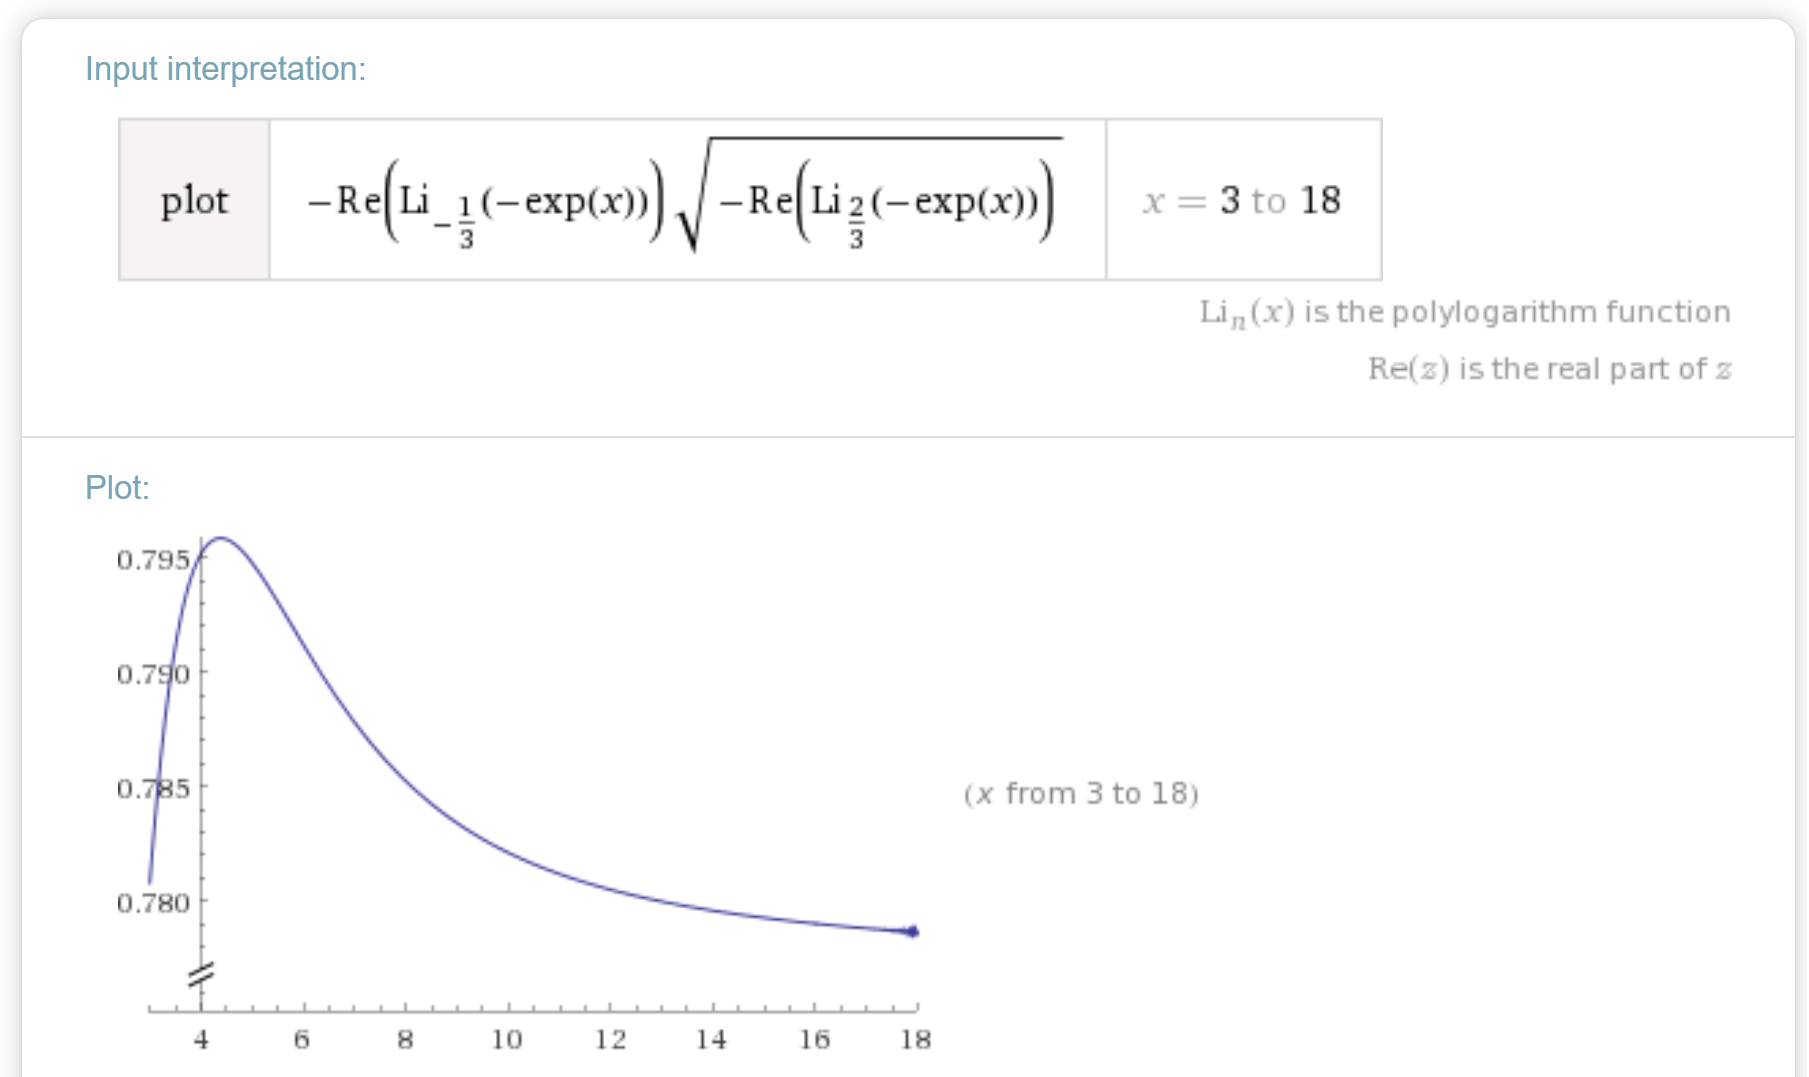
\includegraphics[width=200pt]{polylog_G_less_1}
\end{figure}
\end{document}
